\chapter{Introduction to Graph Theory}

\tikzset{vtx/.style={circle,fill=black,inner sep=1.6pt}}

The second half of the course is about graphs: sets of points (vertices) some pairs of which
are joined (edges). Graphs model networks of all kinds, and many questions about them are
counting questions in disguise.

\section{Definitions}

\begin{definition}[Graph]
A \emph{graph} $G$ is a pair $(V(G), E(G))$ where $V(G)$ is a finite non-empty set of
\emph{vertices} and $E(G)$ is a set of unordered pairs $\{u,v\}$ of distinct vertices, called
\emph{edges}. We write $uv$ for the edge $\{u,v\}$.
\end{definition}

So our graphs have no loops (edges from a vertex to itself) and no multiple edges. (A
\emph{multigraph} allows both; we only use them occasionally.)

\begin{definition}[Adjacency, incidence, degree]
Vertices $u$ and $v$ are \emph{adjacent} (or \emph{neighbours}) if $uv \in E(G)$; the edge $uv$
is \emph{incident} with $u$ and $v$, which are its \emph{ends}. The \emph{degree} $\deg(v)$ of a
vertex $v$ is the number of edges incident with $v$, equivalently the number of neighbours of $v$.
The set of neighbours of $v$ is written $N(v)$.
\end{definition}

\begin{example}
The graph with $V = \{1,2,3,4\}$ and $E = \{12, 13, 14, 23\}$ is drawn below; the degrees are
$\deg(1) = 3$, $\deg(2) = \deg(3) = 2$, $\deg(4) = 1$.
\begin{center}
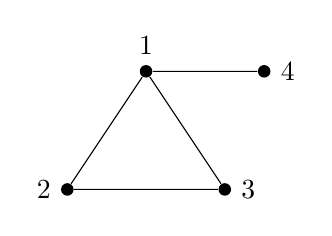
\begin{tikzpicture}
  \node[vtx,label=above:$1$] (1) at (0,1.5) {};
  \node[vtx,label=left:$2$] (2) at (-1,0) {};
  \node[vtx,label=right:$3$] (3) at (1,0) {};
  \node[vtx,label=right:$4$] (4) at (1.5,1.5) {};
  \draw (1)--(2)--(3)--(1)--(4);
\end{tikzpicture}
\end{center}
A drawing is just a picture; the graph is the abstract pair of sets.
\end{example}

\begin{definition}[Subgraph]
$H$ is a \emph{subgraph} of $G$ if $V(H) \subseteq V(G)$ and $E(H) \subseteq E(G)$. It is a
\emph{spanning} subgraph if $V(H) = V(G)$. For $e \in E(G)$, $G - e$ is $G$ with $e$ deleted; for
$v \in V(G)$, $G - v$ is $G$ with $v$ and all edges incident with $v$ deleted.
\end{definition}

\section{Isomorphism}

\begin{definition}[Isomorphism]
Graphs $G$ and $H$ are \emph{isomorphic}, written $G \cong H$, if there is a bijection
$f : V(G) \to V(H)$ such that $uv \in E(G)$ if and only if $f(u)f(v) \in E(H)$; that is,
$E(H) = \{f(u)f(v) : uv \in E(G)\}$. Such an $f$ is an \emph{isomorphism}.
\end{definition}

Isomorphic graphs are ``the same graph with different names''. To show two graphs are
isomorphic, exhibit an isomorphism and check every edge. To show they are \emph{not}, find a
property preserved by isomorphisms that one has and the other lacks: number of vertices or
edges, the degree sequence, number of triangles, being connected, being bipartite, containing a
cycle of a given length, and so on.

\begin{example}
The two drawings below are both the $4$-cycle: $f(a)=1, f(b)=2, f(c)=3, f(d)=4$ is an
isomorphism from the left graph (edges $ab, bc, cd, da$) to the right graph (edges
$12, 23, 34, 41$), even though the right drawing has crossing edges.
\begin{center}
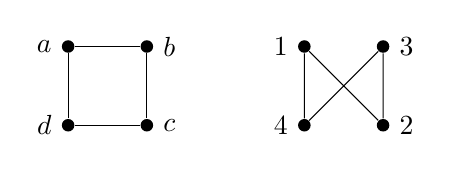
\begin{tikzpicture}
  \node[vtx,label=left:$a$] (a) at (0,1) {};
  \node[vtx,label=right:$b$] (b) at (1,1) {};
  \node[vtx,label=right:$c$] (c) at (1,0) {};
  \node[vtx,label=left:$d$] (d) at (0,0) {};
  \draw (a)--(b)--(c)--(d)--(a);
  \begin{scope}[xshift=3cm]
  \node[vtx,label=left:$1$] (1) at (0,1) {};
  \node[vtx,label=right:$2$] (2) at (1,0) {};
  \node[vtx,label=right:$3$] (3) at (1,1) {};
  \node[vtx,label=left:$4$] (4) at (0,0) {};
  \draw (1)--(2)--(3)--(4)--(1);
  \end{scope}
\end{tikzpicture}
\end{center}
\end{example}

\begin{aside}
There are $2^{\binom{n}{2}}$ graphs on a fixed vertex set $[n]$ (each of the $\binom n2$ pairs
is an edge or not), but far fewer isomorphism classes: for $n=4$ there are $64$ labelled graphs
but only $11$ graphs up to isomorphism.
\end{aside}

\begin{example}
Equal degree sequences do not imply isomorphism. Both graphs below are $2$-regular with $6$
vertices and $6$ edges, but the left one is connected and the right one is not (equivalently:
the right one contains a triangle and the left one does not), so they are not isomorphic.
\begin{center}
\begin{tikzpicture}
  \foreach \i in {1,...,6} \node[vtx] (c\i) at ({60*\i}:1) {};
  \draw (c1)--(c2)--(c3)--(c4)--(c5)--(c6)--(c1);
  \node at (0,-1.5) {$C_6$};
  \begin{scope}[xshift=3.5cm]
    \foreach \i in {1,2,3} \node[vtx] (t\i) at ({120*\i+90}:0.7) {};
    \draw (t1)--(t2)--(t3)--(t1);
    \foreach \i in {1,2,3} \node[vtx] (s\i) at ($({120*\i+90}:0.7)+(2,0)$) {};
    \draw (s1)--(s2)--(s3)--(s1);
    \node at (1,-1.5) {two disjoint triangles};
  \end{scope}
\end{tikzpicture}
\end{center}
\end{example}

\section{The handshake lemma}

\begin{theorem}[Handshake lemma]
For every graph $G$, $\displaystyle\sum_{v \in V(G)}\deg(v) = 2\abs{E(G)}$.
\end{theorem}
\begin{proof}
Count the pairs $(v, e)$ with $v \in V(G)$, $e \in E(G)$ and $v \in e$. Summing over vertices,
vertex $v$ is in $\deg(v)$ such pairs. Summing over edges, each edge has exactly two ends. So
\[
\sum_{v\in V(G)}\deg(v) = \sum_{v \in V(G)}\abs{\{e\in E(G) : v \in e\}}
= \sum_{e\in E(G)}\abs{\{v : v\in e\}} = \sum_{e \in E(G)} 2 = 2\abs{E(G)}.
\]
\end{proof}

\begin{corollary}
Every graph has an even number of vertices of odd degree.
\end{corollary}
\begin{proof}
The sum of all degrees is even, and the vertices of even degree contribute an even amount.
\end{proof}

\begin{corollary}
The average degree of $G$ is $2\abs{E(G)}/\abs{V(G)}$.
\end{corollary}

\begin{example}
Is there a graph with degree sequence $3,3,3,3,3$? No: five odd-degree vertices. Is there one
with $3,3,3,3$? Yes, $K_4$, which has $\frac{4\cdot3}{2} = 6$ edges.
\end{example}

\section{Regular and complete graphs}

\begin{definition}[Regular]
A graph is \emph{$k$-regular} if every vertex has degree $k$. By the handshake lemma a
$k$-regular graph on $p$ vertices has $kp/2$ edges, so $kp$ must be even.
\end{definition}

\begin{definition}[Special graphs]
\begin{itemize}
  \item The \emph{complete graph} $K_n$ has $n$ vertices, every pair adjacent: it is
        $(n-1)$-regular with $\binom{n}{2}$ edges.
  \item The \emph{empty graph} on $n$ vertices has no edges ($0$-regular).
  \item The \emph{path} $P_n$ has vertices $v_1,\dots,v_n$ and edges $v_iv_{i+1}$ for $1\le i<n$
        (so $n-1$ edges; some books index paths by their number of edges instead).
  \item The \emph{cycle} $C_n$ ($n \ge 3$) is $P_n$ plus the edge $v_nv_1$: $2$-regular with $n$ edges.
\end{itemize}
\end{definition}

\begin{center}
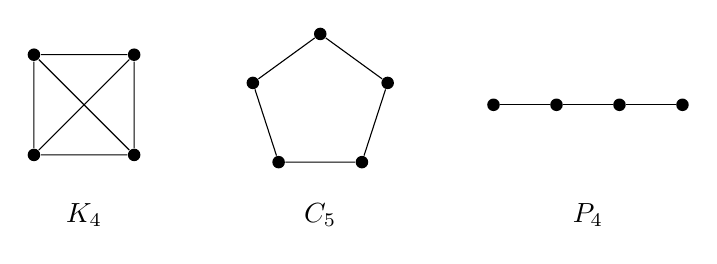
\begin{tikzpicture}
  % K4
  \foreach \i in {1,...,4} \node[vtx] (k\i) at ({90*\i+45}:0.9) {};
  \draw (k1)--(k2)--(k3)--(k4)--(k1)--(k3) (k2)--(k4);
  \node at (0,-1.4) {$K_4$};
  % C5
  \begin{scope}[xshift=3cm]
  \foreach \i in {1,...,5} \node[vtx] (c\i) at ({72*\i+18}:0.9) {};
  \draw (c1)--(c2)--(c3)--(c4)--(c5)--(c1);
  \node at (0,-1.4) {$C_5$};
  \end{scope}
  % P4
  \begin{scope}[xshift=5.2cm]
  \foreach \i in {1,...,4} \node[vtx] (p\i) at (0.8*\i-0.8,0) {};
  \draw (p1)--(p2)--(p3)--(p4);
  \node at (1.2,-1.4) {$P_4$};
  \end{scope}
\end{tikzpicture}
\end{center}

\section{Bipartite graphs}

\begin{definition}[Bipartite]
A graph $G$ is \emph{bipartite} if $V(G)$ can be partitioned into two sets $X$ and $Y$
($V = X\cup Y$, $X \cap Y = \emptyset$) such that every edge has one end in $X$ and one end in
$Y$. The pair $(X,Y)$ is a \emph{bipartition}.
\end{definition}

\begin{example}
Empty graphs, paths and even cycles are bipartite: for $C_{2m}$ or $P_n$, put the odd-numbered
vertices in $X$ and the even-numbered ones in $Y$. Every subgraph of a bipartite graph is bipartite
(restrict the bipartition).
\end{example}

\begin{proposition}
Odd cycles are not bipartite. Consequently a graph containing an odd cycle as a subgraph is not
bipartite.
\end{proposition}
\begin{proof}
In $C_{2m+1}$ with vertices $v_1, \dots, v_{2m+1}$, if $v_1 \in X$ then going around the cycle
the vertices must alternate $X, Y, X, \dots$, so $v_i \in X$ iff $i$ is odd. But then $v_{2m+1}$
and $v_1$ are adjacent and both in $X$. The second statement follows since subgraphs of
bipartite graphs are bipartite.
\end{proof}

We will see in the chapter on trees that the converse holds: a graph is bipartite if and only if
it has no odd cycle.

\begin{proposition}
If $G$ is bipartite with bipartition $(X,Y)$, then
$\displaystyle \abs{E(G)} = \sum_{v\in X}\deg(v) = \sum_{v\in Y}\deg(v)$.
\end{proposition}
\begin{proof}
Each edge has exactly one end in $X$, so summing degrees over $X$ counts each edge exactly once.
Similarly for $Y$.
\end{proof}

\begin{definition}[Complete bipartite graph]
$K_{p,q}$ has bipartition $(X,Y)$ with $\abs{X} = p$, $\abs{Y} = q$, and every vertex of $X$
adjacent to every vertex of $Y$. It has $p+q$ vertices; vertices in $X$ have degree $q$ and
vertices in $Y$ have degree $p$; it has $pq$ edges.
\end{definition}

\begin{center}
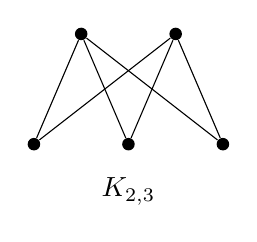
\begin{tikzpicture}
  \foreach \i in {1,2} \node[vtx] (x\i) at (1.2*\i,1.4) {};
  \foreach \j in {1,2,3} \node[vtx] (y\j) at (1.2*\j-0.6,0) {};
  \foreach \i in {1,2} \foreach \j in {1,2,3} \draw (x\i)--(y\j);
  \node at (1.8,-0.6) {$K_{2,3}$};
\end{tikzpicture}
\end{center}

\section{The $n$-cube}

\begin{definition}[$n$-cube]
The \emph{$n$-cube} $Q_n$ has as vertices the $2^n$ binary strings of length $n$, with two
strings adjacent iff they differ in exactly one position.
\end{definition}

\begin{proposition}
$Q_n$ has $2^n$ vertices, is $n$-regular, has $n2^{n-1}$ edges, and is bipartite.
\end{proposition}
\begin{proof}
A string has exactly $n$ neighbours (flip one of its $n$ bits), so $Q_n$ is $n$-regular and by
the handshake lemma has $n2^n/2 = n2^{n-1}$ edges. Let $X$ be the strings with an even number of
$1$s and $Y$ those with an odd number. Flipping one bit changes the number of $1$s by one, so
every edge joins $X$ to $Y$.
\end{proof}

\begin{center}
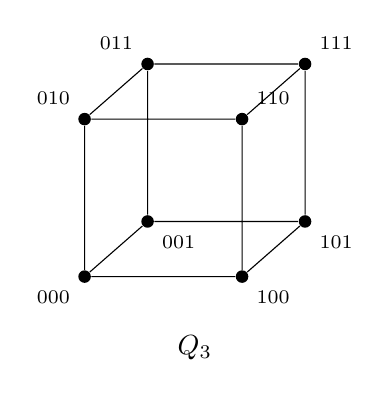
\begin{tikzpicture}[every label/.style={font=\scriptsize}]
  \node[vtx,label=below left:$000$] (a) at (0,0) {};
  \node[vtx,label=below right:$100$] (b) at (2,0) {};
  \node[vtx,label=above left:$010$] (c) at (0,2) {};
  \node[vtx,label=above right:$110$] (d) at (2,2) {};
  \node[vtx,label=below right:$001$] (e) at (0.8,0.7) {};
  \node[vtx,label=below right:$101$] (f) at (2.8,0.7) {};
  \node[vtx,label=above left:$011$] (g) at (0.8,2.7) {};
  \node[vtx,label=above right:$111$] (h) at (2.8,2.7) {};
  \draw (a)--(b)--(d)--(c)--(a) (e)--(f)--(h)--(g)--(e)
        (a)--(e) (b)--(f) (c)--(g) (d)--(h);
  \node at (1.4,-0.9) {$Q_3$};
\end{tikzpicture}
\end{center}

Redrawing $Q_3$ with the even-weight strings on top and the odd-weight strings below makes the
bipartition visible: every edge goes between the two rows.
\begin{center}
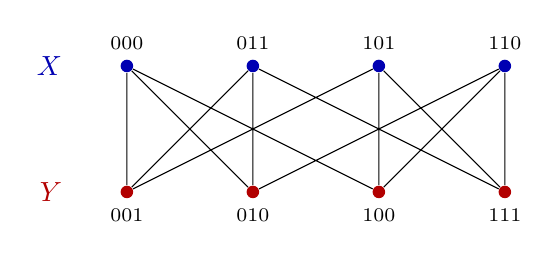
\begin{tikzpicture}[every label/.style={font=\scriptsize}]
  \foreach \s [count=\i] in {000,011,101,110} \node[vtx,fill=blue!70!black,label=above:$\s$] (x\s) at (1.6*\i,1.6) {};
  \foreach \s [count=\i] in {001,010,100,111} \node[vtx,fill=red!70!black,label=below:$\s$] (y\s) at (1.6*\i,0) {};
  \draw (x000)--(y001) (x000)--(y010) (x000)--(y100)
        (x011)--(y001) (x011)--(y010) (x011)--(y111)
        (x101)--(y001) (x101)--(y100) (x101)--(y111)
        (x110)--(y010) (x110)--(y100) (x110)--(y111);
  \node[left,blue!70!black] at (0.9,1.6) {$X$};
  \node[left,red!70!black] at (0.9,0) {$Y$};
\end{tikzpicture}
\end{center}

\section{Summary}
\begin{itemize}
  \item A graph is a pair $(V,E)$ with $E$ a set of $2$-subsets of $V$; isomorphism is a
        bijection preserving adjacency.
  \item Handshake lemma: $\sum\deg(v) = 2\abs{E}$; the number of odd-degree vertices is even.
  \item $K_n$: $\binom n2$ edges; $C_n$: $2$-regular; $K_{p,q}$: $pq$ edges; $Q_n$: $2^n$ vertices,
        $n$-regular, $n2^{n-1}$ edges.
  \item Bipartite: every edge crosses $(X,Y)$; even cycles are bipartite, odd cycles are not.
\end{itemize}
